To generate dynamically balanced walking trajectories for humanoid robots and to let them navigate the environment autonomously, there are several posed challenges that we need to cover. As the logical starting point, in section \ref{sec::31_hm} - Humanoid Walking, we want to address the real time generation of walking trajectories for humanoid robots first, and then think of ways to replace the human user by an artificial agent in the control loop. As discussed in section \ref{sec::2_sota} - State of The Art, there are several ways to achieve this, but of particular interest to us are novel methods that evolved from the toolbox of machine learning techniques. Center to these new methods will be neural nets that we will try to train on solving the task of autonomous navigation in different ways, as shown in section \ref{sec::32_ml} - Machine Learning.
\begin{figure}[h]
	\centering
	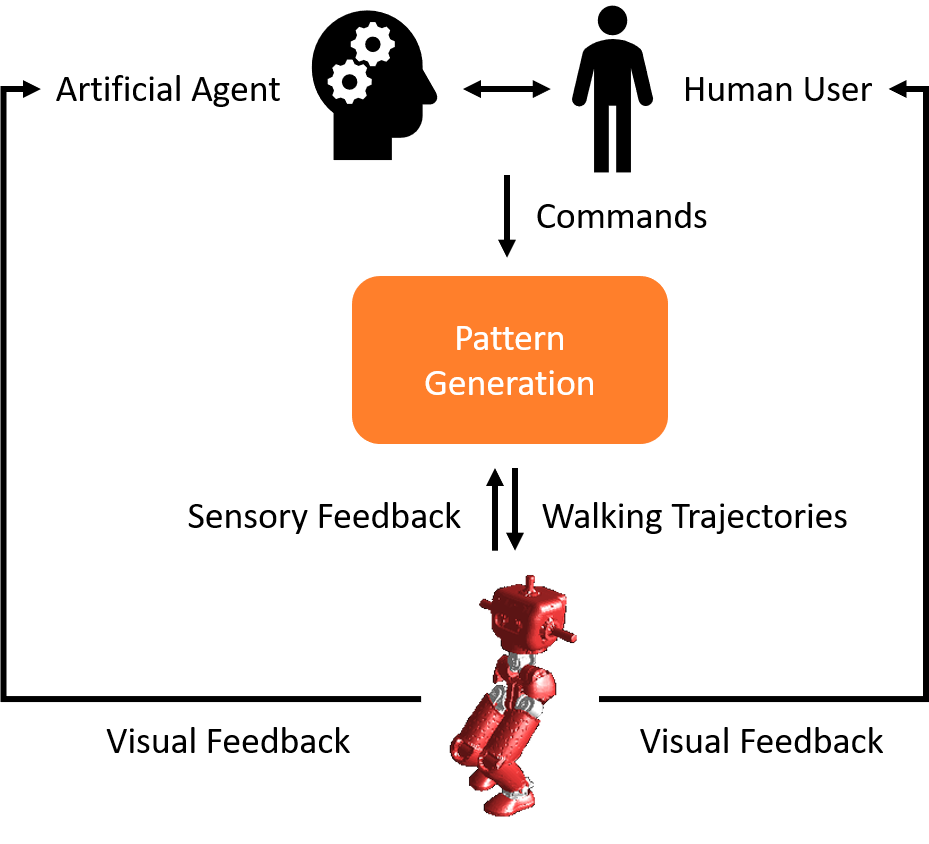
\includegraphics[scale=.5]{chapters/03_background/img/control_loop.png}
	\caption{\label{fig::3_cl} Proposed control loop to navigate the robot with either a human user or an artificial agent.}
\end{figure}